\documentclass[11pt,a4paper]{article}

\usepackage[utf8]{inputenc}
\usepackage[T1]{fontenc}
\usepackage[a4paper,margin=1in]{geometry}
\usepackage{tabularx}
\usepackage{array}
\usepackage{booktabs}
\usepackage{enumitem}
\usepackage{graphicx}
\graphicspath{{./}{../documentation/}}
\usepackage[hidelinks]{hyperref}
\usepackage{fancyhdr}
\usepackage{setspace}
\usepackage{listings}
\usepackage{xcolor}
% Highlight macros (soul + colortbl) — remove \new wrapper + \rowcolor lines for an unhighlighted PDF
\usepackage{soul}
\usepackage{colortbl}
\sethlcolor{yellow}
\newcommand{\new}[1]{\hl{#1}}

% ── Code listing style ────────────────────────────────
\lstdefinestyle{pysnippet}{
  language=Python,
  basicstyle=\ttfamily\footnotesize,
  keywordstyle=\bfseries\color{blue!70!black},
  commentstyle=\itshape\color{gray},
  stringstyle=\color{red!60!black},
  numbers=left,numberstyle=\tiny\color{gray},numbersep=5pt,
  frame=single,framerule=0.4pt,
  breaklines=true,breakatwhitespace=false,
  showstringspaces=false,
  aboveskip=0.6em,belowskip=0.4em,
  xleftmargin=1.5em,
}

% ── Paragraph and spacing ──────────────────────────────
\setlength{\parindent}{0pt}
\setlength{\parskip}{0.5\baselineskip}
\setlength{\tabcolsep}{5pt}
\renewcommand{\arraystretch}{1.15}
\onehalfspacing

% ── Page headers and footers ───────────────────────────
\pagestyle{fancy}
\fancyhf{}
\fancyhead[L]{\small\textit{System Documentation}}
\fancyhead[R]{\small\textit{Group 9 -- Five Guys}}
\fancyfoot[C]{\thepage}
\renewcommand{\headrulewidth}{0.4pt}
\renewcommand{\footrulewidth}{0pt}

% ── Section numbering depth ────────────────────────────
\setcounter{secnumdepth}{3}
\setcounter{tocdepth}{3}

\begin{document}

% ── Title block ────────────────────────────────────────
\begin{center}
{\LARGE \textbf{System Documentation}}\\[0.4em]
{\Large Business Sustainability Management Platform}\\[0.6em]
{\large Group 9 --- Five Guys}
\end{center}

\vspace{0.4em}
\hrule
\vspace{0.6em}
\begin{tabular}{@{}ll}
\textbf{Document Type:}  & System Documentation \\
\textbf{Filename:}       & Group\_9\_system\_documentation.pdf \\
\textbf{Project Focus:}  & Web-based ESG and sustainability management platform \\
\textbf{Date:}           & \today \\
\end{tabular}
\vspace{0.4em}
\hrule

\vspace{1em}
\tableofcontents
\newpage

\section*{Abstract}
\addcontentsline{toc}{section}{Abstract}
This document presents the system documentation for the Business Sustainability Management Platform developed by Group 9. The platform is intended to support practical ESG management in a multi-store business setting through integrated carbon tracking, waste management, sustainability reporting, alert monitoring, and governance-related ESG functions. Instead of relying on separate spreadsheets or isolated reports, the system provides a browser-based workflow that supports structured record keeping, clearer data visibility, and role-sensitive access.

The implemented system combines operational sustainability functions with higher-level governance features. Core modules include dashboard analytics, carbon and waste data recording, sustainability report generation, alert threshold management, supplier ESG assessment, ESG policy management, staff training records, compliance scoring, anomaly detection, user management, and audit logging. The platform also includes supporting functions such as OCR-assisted bill scanning, PDF export, mock fallback strategies for demonstration stability, and multi-role access control for administrators, headquarters managers, regional managers, and store staff.

Technically, the platform is implemented using Flask, Jinja2, Bootstrap, MySQL, and several supporting tools including Flask-Mail and WeasyPrint. In its current form, the system is complete enough to be tested and demonstrated, while still being lightweight enough for browser-based use and academic evaluation.

\new{Highlighted text in this document marks the substantive technical capabilities of the delivered platform. The carbon and waste modules expose CSV / Excel import and export endpoints powered by \texttt{pandas}; the alert subsystem is wired to a real Mailtrap SMTP sandbox with a deterministic mock fallback; the report generator chooses between a DeepSeek-backed AI commentary and a rule-based template generator and persists the chosen narrative source on each report; the anomaly module includes an LLM insight layer backed by a four-state human-triage workflow (Open, Reviewed, False Positive, Resolved); the OCR endpoint handles both image (Pillow + pytesseract) and PDF (pdfplumber) inputs through a three-layer extract / regex / mock pipeline; and a dedicated geographic map module visualises store-level ESG performance through Leaflet with MarkerCluster and heat-map plug-ins. The platform is deployed onto a UCD-provided Ubuntu virtual machine running Nginx, Gunicorn, and systemd, with a role-aware dashboard providing an end-to-end ESG management workflow.}

\section{Introduction}

\subsection{Project Background}
Environmental, Social, and Governance (ESG) concerns have become more important in business management~\cite{eccles2014}, especially for organisations that operate across multiple physical locations and need more consistent sustainability oversight. In restaurant and coffee-shop style businesses, day-to-day sustainability work often includes repetitive operational tasks such as recording energy use, tracking waste generation, monitoring recycling performance, and preparing summary reports for management review. In many cases, however, these tasks are still handled through separate spreadsheets, manually prepared documents, or informal communication between branches. This makes long-term monitoring harder and can also reduce the transparency of sustainability claims.

The Business Sustainability Management Platform was developed to respond to this problem in a practical way. The project focuses on building a web-based platform that can bring sustainability-related operational data and governance functions into one interface. By integrating data collection, analytics, reporting, alerts, and ESG management, the system aims to improve traceability, consistency, and visibility for sustainability work across multiple stores. This direction is consistent with the reporting principles outlined in the GRI Standards~\cite{gri2021} and the UN Sustainable Development Goal~12~\cite{un_sdg12}.

\subsection{Problem Statement}
Before this platform was developed, sustainability-related activities in the target business scenario were difficult to monitor in a consistent and structured way. Carbon records, waste records, and reporting outputs could be created, but they were not easy to standardise across different stores. Management therefore lacked an efficient way to compare branch performance, detect unusual data patterns, monitor reporting coverage, or evaluate suppliers from an ESG perspective. At the same time, different users needed different permissions, which meant that a realistic solution required not only data-entry pages but also a clear access-control model.

The system was therefore designed to address three linked problems. First, it needed to provide a reliable operational layer for recording carbon and waste data. Second, it needed to turn these data into useful management outputs such as dashboards, reports, and alerts. Third, it needed to extend beyond operational monitoring into governance-oriented ESG management through supplier assessment, policy management, compliance scoring, and audit support.

\subsection{Project Objectives}
The main objective of the project is to create a practical ESG management platform that supports both sustainability operations and management decision-making. To achieve this objective, the project was designed around several concrete goals:

\begin{itemize}[leftmargin=1.4em,itemsep=2pt,topsep=2pt]
    \item provide structured carbon and waste tracking workflows for different business roles;
    \item support dashboard-based data visualisation and summary analysis;
    \item enable sustainability report generation and PDF export;
    \item provide alert and notification functions for management monitoring;
    \item integrate ESG governance features such as supplier assessment and policy management;
    \item support administrative and assurance functions including compliance scoring, anomaly detection, user management, and audit logging.
\end{itemize}

\subsection{Project Planning and Scope Evolution}
The project began with core sustainability functions---carbon tracking, waste management, dashboard review, and reporting---and gradually expanded through iterative refinement. The current version includes supplier ESG scorecard assessment, ESG policy management, compliance evaluation, anomaly detection, user administration, audit logging, OCR-assisted input, and alert-based monitoring, reflecting both the original sustainability direction and the later integration of governance and assurance functions.

\subsection{Target Users}
The platform is designed for four main user roles: administrators, headquarters managers, regional managers, and store staff. These roles differ in both their responsibilities and their access scope. Administrators and headquarters managers can oversee company-wide data and configuration. Regional managers focus on the stores within their region. Store staff primarily create and manage operational records for their own store. This role distinction shaped both the backend access-control logic and the frontend page visibility of the final system.

\section{Technical Implementation}

\subsection{System Architecture and Technology Stack}
The platform follows a three-tier client-server architecture (presentation, application, and data layer) implemented with Flask~\cite{flask2023} and organised through modular blueprints, one per business area. \new{The application registers fifteen blueprints in \texttt{backend/app.py}: \texttt{auth}, \texttt{dashboard}, \texttt{carbon}, \texttt{waste}, \texttt{report}, \texttt{alert}, \texttt{ocr}, \texttt{audit}, \texttt{admin}, \texttt{anomaly}, \texttt{training}, \texttt{compliance}, \texttt{supplier}, \texttt{policy}, and \texttt{map}. Governance-oriented modules added later (supplier scorecard, policy management, anomaly detection, compliance scoring, geographic map) were integrated without restructuring the original operational blueprints.}

\begin{figure}[h]
\centering
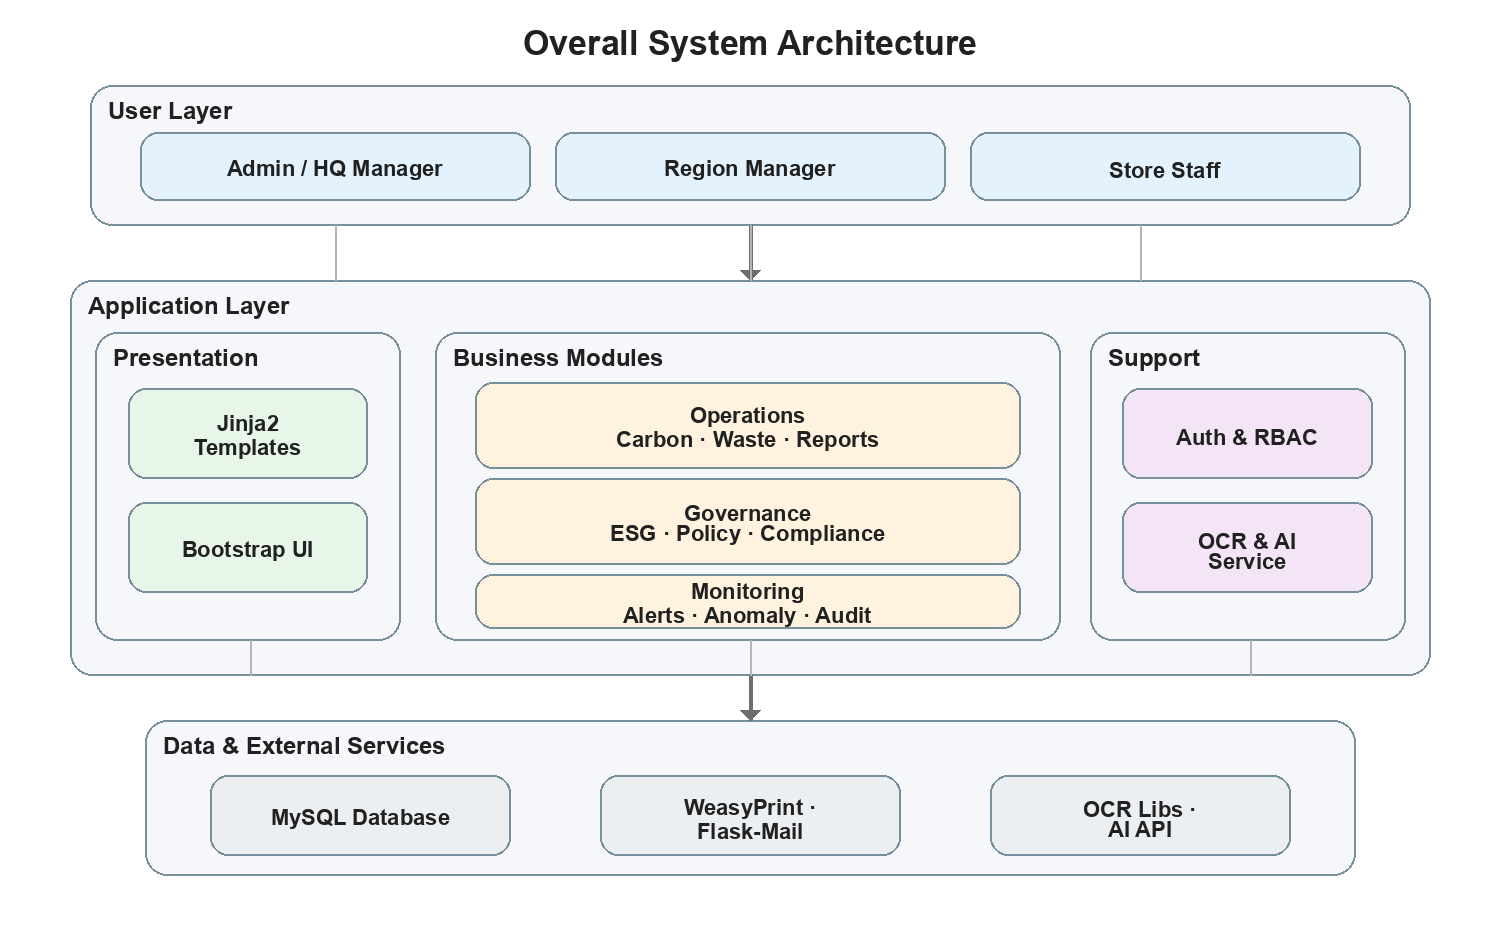
\includegraphics[width=0.92\linewidth]{figures/system_architecture_compact.png}
\caption{Overall System Architecture of the Business Sustainability Management Platform}
\end{figure}

\begin{figure}[h]
\centering
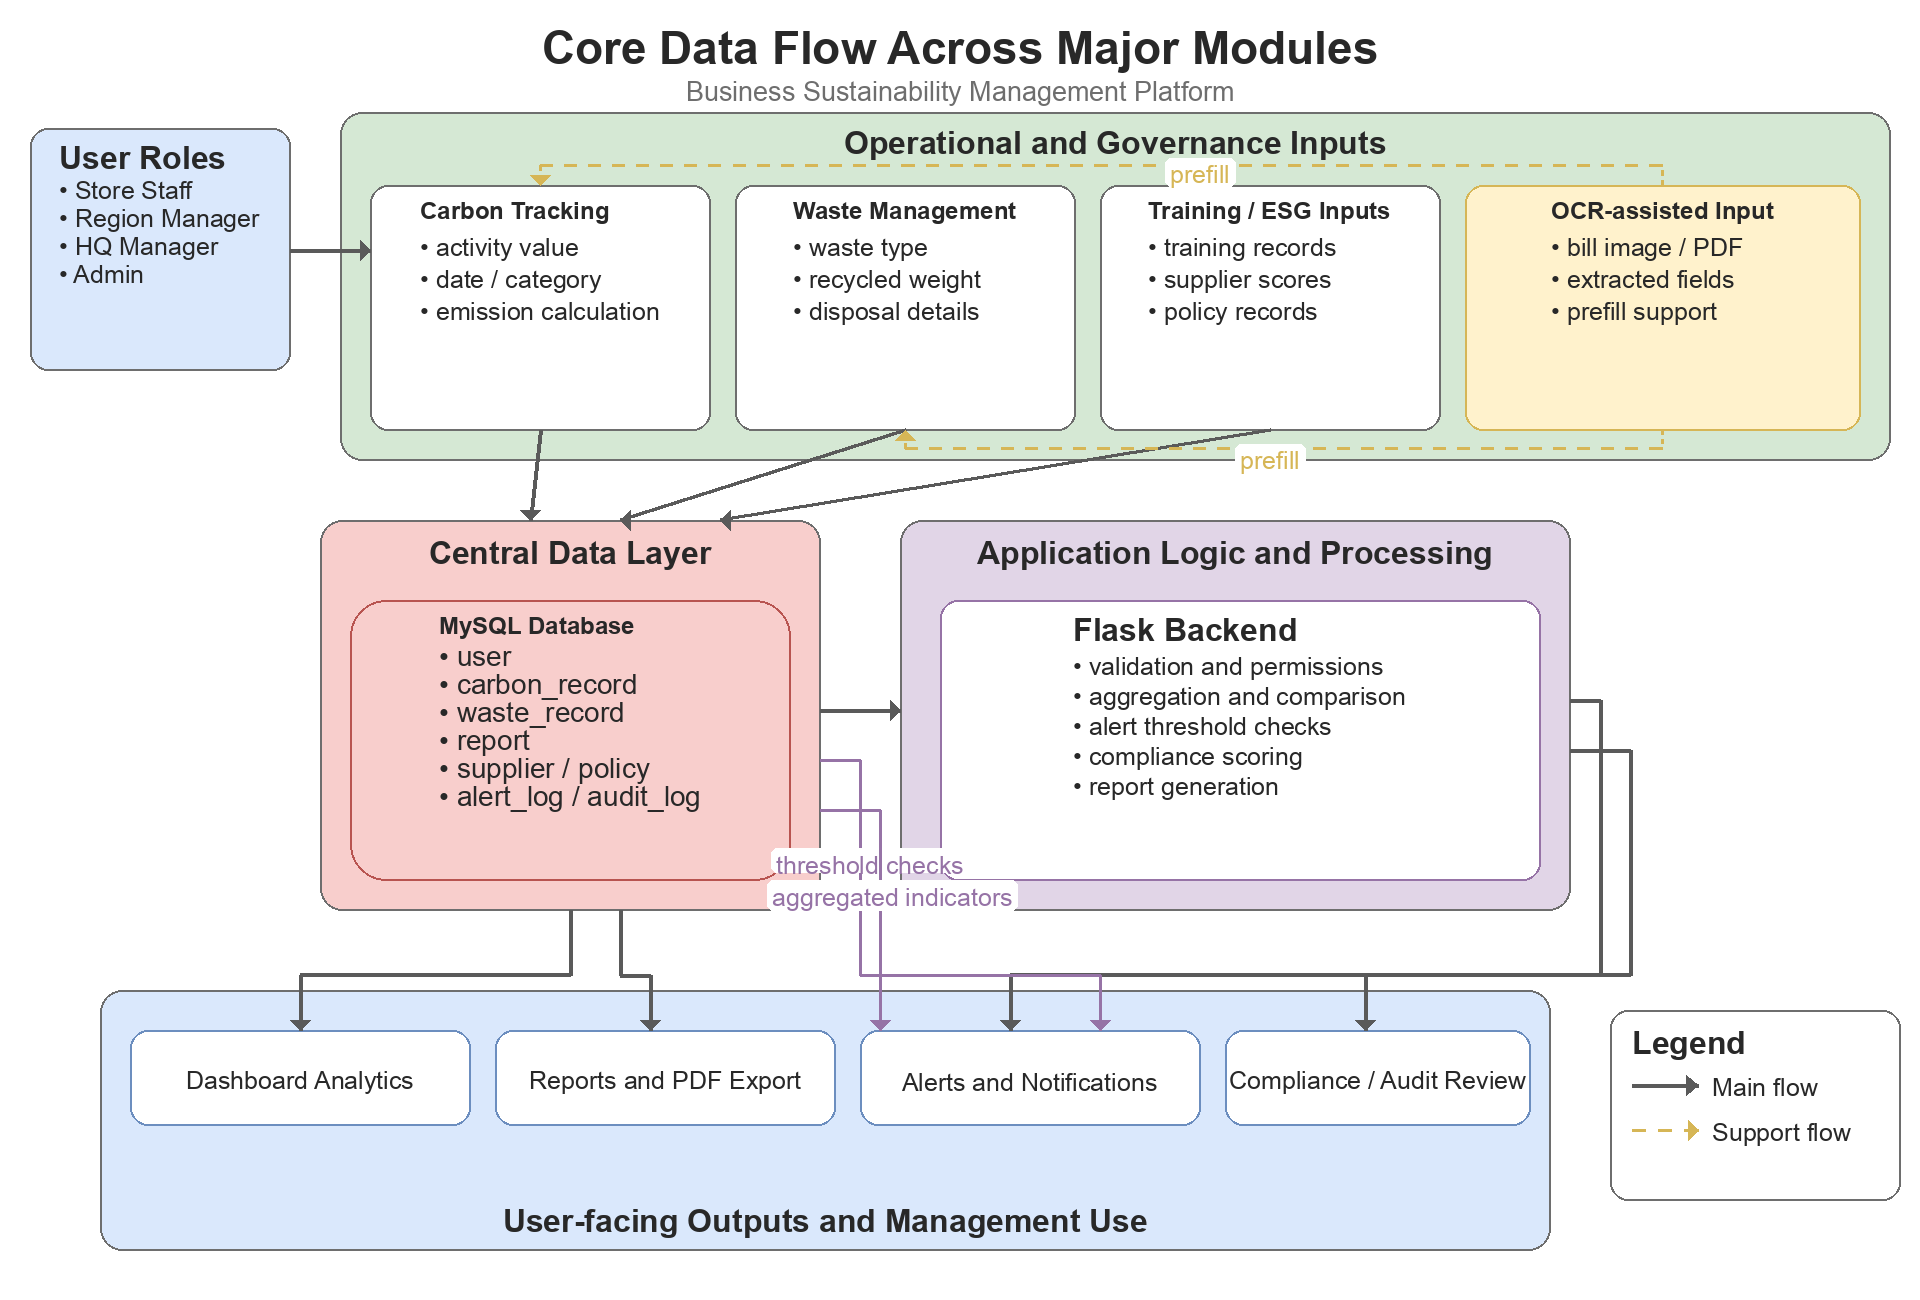
\includegraphics[width=0.95\linewidth]{figures/system_core_data_flow.png}
\caption{Core Data Flow Across Major Modules}
\end{figure}

The frontend uses Jinja2 templates with Bootstrap~\cite{bootstrap}, providing server-rendered pages plus lightweight dynamic behaviour through shared headers, sidebars, and reusable forms / tables / charts. MySQL~\cite{mysql2024} stores all operational, governance, identity, alert, report, and audit data. Flask-Mail handles notifications and WeasyPrint~\cite{weasyprint} produces PDF reports. The platform additionally integrates \texttt{pytesseract}~\cite{tesseract} with \texttt{Pillow} and \texttt{pdfplumber} for OCR-assisted bill scanning, \texttt{pandas}~\cite{pandas2024} for bulk CSV / Excel parsing, the DeepSeek API~\cite{deepseek2024} for AI commentary on reports and anomaly insights, and Leaflet~\cite{leaflet2024} 1.9.4 with MarkerCluster~\cite{markercluster} and Heat plug-ins for the store map. \new{Each external dependency follows the same fallback principle---if the service or library is unavailable, the platform degrades to a deterministic mock path so demonstrations remain reproducible.}

\begin{table}[h]
\centering
\scriptsize\sloppy
\begin{tabularx}{\linewidth}{@{}>{\raggedright\arraybackslash}p{0.25\linewidth}p{0.10\linewidth}X@{}}
\toprule
\textbf{Table / View} & \textbf{Category} & \textbf{Role in the System} \\
\midrule
company, region, store & Organisation & Define the three-level hierarchy (HQ $\rightarrow$ region $\rightarrow$ store) used for data isolation and scope-based access control\new{; the \texttt{store} table additionally carries \texttt{latitude}/\texttt{longitude} columns for the geographic map module} \\
user & Identity & Store credentials, role (admin / hq\_manager / region\_manager / store\_staff), and organisational scope for session-based authentication \\
emission\_factor & Reference & Pre-seeded lookup of emission coefficients by category and sub-type, used to convert activity values into carbon kg during record creation \\
carbon\_record & Operations & Record-level carbon data including activity value, calculated emissions, category, store, and date; feeds dashboards, reports, alerts, and comparisons \\
waste\_category & Reference & Enumeration of waste types with recyclability flags; referenced by waste records for classification \\
waste\_record & Operations & Record-level waste data including weights, disposal method, and store; contributes to recycling analysis, compliance, and reporting \\
report & Reporting & Persisted sustainability report with aggregated carbon and waste summaries, SDG indicators, optional AI commentary, and PDF export support \\
sdg\_goal, company\_sdg & Governance & UN SDG reference data and per-company alignment tracking with target values and progress percentages \\
alert\_threshold & Monitoring & Configurable metric thresholds at company / region / store level for waste recycling rate, carbon MoM growth, and daily waste weight \\
alert\_log & Monitoring & Triggered alert records with metric snapshots, read-state management, and optional email notification tracking \\
audit\_log & Audit & Immutable log of user actions (login, create, update, delete, export) for traceability and compliance review \\
supplier & Governance & Supplier records with a 16-indicator ESG scorecard across carbon, waste, ethics, and reporting dimensions; rule-based scoring \\
esg\_policy & Governance & Internal ESG policy documents with versioning, status lifecycle (draft / active / archived), and category tagging \\
\rowcolor{yellow!40}
training\_record & Operations & Sustainability training entries (course type, duration, score, completion date, status) used by training summaries and the compliance score \\
\rowcolor{yellow!40}
anomaly\_review & Monitoring & Persistent triage state machine for detected anomalies (Open / Reviewed / False Positive / Resolved) preserved across re-detection runs \\
\midrule
v\_carbon\_monthly\_summary,\newline v\_waste\_monthly\_* & View & Monthly aggregated carbon and waste summaries by store; used for dashboard charts and MoM trends \\
v\_store\_carbon\_summary,\newline v\_store\_waste\_summary & View & Store-level monthly totals used for alert threshold evaluation (MoM growth, recycling rate) \\
\bottomrule
\end{tabularx}
\caption{Key Database Entities and Their Roles}
\end{table}

\subsection{Authentication and Role-Based Access Control}
The system uses username-and-password authentication with server-side session management. After successful login, the backend stores key identity and scope information in the session, including the current user's role, company, region, and store context. This design fits a server-rendered Flask application because it keeps access control logic close to the business routes and avoids exposing sensitive authorisation state on the client side, in line with secure session management practices recommended by OWASP~\cite{owasp2021}.

Role-based access control is implemented as a core design principle. Administrators and headquarters managers access company-wide data and configuration, regional managers are limited to their assigned region, and store staff are restricted to their own store. Within modules, store staff are subject to tighter edit and delete windows, while higher-level roles can configure alerts, manage users, access compliance views, and use governance features such as supplier ESG assessment and policy management. This multi-layered approach reflects real reporting hierarchies and operational accountability, making access control a structural feature of the system rather than a narrow security add-on.

\new{Implementation is centralised in a single auth-helper module that exposes three reusable building blocks. The \texttt{@login\_required} decorator redirects unauthenticated visitors to the login page. The \texttt{@role\_required(*roles)} decorator restricts a route to one or more of the four system roles. The \texttt{get\_accessible\_store\_ids()} helper returns the exact list of store IDs the current session is allowed to touch, derived from the role-scope mapping (admin and HQ manager: all company stores; region manager: stores in the assigned region; store staff: only the bound store). Every list, aggregation, export and chart query funnels through this helper, so data isolation is enforced once at the query layer rather than re-implemented per page. Passwords are stored as \texttt{werkzeug} PBKDF2 hashes with per-account salts and are never logged or returned to the client, in keeping with the OWASP password-storage guidance referenced above.}

\begin{table}[h]
\centering
\scriptsize
\begin{tabularx}{\linewidth}{@{}p{0.14\linewidth}p{0.15\linewidth}p{0.14\linewidth}p{0.11\linewidth}p{0.12\linewidth}X@{}}
\toprule
\textbf{Role} & \textbf{Scope} & \textbf{Carbon/Waste} & \textbf{Reports} & \textbf{Alerts} & \textbf{Key Management Functions} \\
\midrule
Admin & Company-wide & Full CRUD + CSV import/export & Full & Config + review & Users, audit, compliance, anomaly review, ESG governance, training, map \\
HQ Manager & Company-wide & Full CRUD + CSV import/export & Full & Config + review & Compliance, anomaly review, ESG governance, company users, training, map \\
Region Manager & Assigned region & Regional access + CSV export & Regional & Review only & Compliance, anomaly review (region scope), training, map (region) \\
Store Staff & Own store only & Own-store with time limits & Limited use & View only & No admin / governance / anomaly config; map and training records limited to own store \\
\bottomrule
\end{tabularx}
\caption{Role-Based Access Scope and Functional Permissions}
\end{table}

\subsection{Dashboard and Data Visualisation}
The dashboard module transforms recorded operational data into summary indicators and management-oriented visualisations. It provides an overview of total carbon emissions, total waste, recycling performance, and report volume, while also supporting chart-based review of carbon trends, waste composition, and category-level breakdowns. Drilldown support enables users to move from aggregated company or regional indicators to more specific store-level views. Charts are rendered with ECharts~5~\cite{echarts}. \new{The dashboard exposes a monthly carbon trend line chart, a waste-category composition pie, a region-by-region carbon comparison bar chart, and a recycling-rate trend overlay; all chart series are populated through \texttt{/api/dashboard/*} endpoints that share the same \texttt{get\_accessible\_store\_ids()} filter as the rest of the platform, so what a user sees on the dashboard is consistent with what they can see in the underlying record lists.}

An additional analytical layer connects the dashboard to SDG 12 related indicators, including waste recovery, carbon efficiency, reporting coverage, and store data coverage. This makes the dashboard not only a display page but also a compact decision-support surface for sustainability oversight.

\new{The dashboard adopts a role-aware layout. Below the shared KPI summary cards, the page renders a different set of secondary cards depending on the user's role, so each role lands directly on the information that is most relevant to their daily work rather than on a generic overview. Store staff see an \emph{Open Alerts} card that lists every unread alert on their own store; region managers see two leaderboards (year-to-date recycling rate ranking and year-to-date carbon emissions ranking) for the stores in their region; headquarters managers see a three-pane \emph{Risk Watch} (high-alert stores, carbon-spike stores, and silent stores with no recent data submission); administrators see a \emph{System Health} card with active-user counts, audit activity over the last twenty-four hours, and outstanding alerts across the platform. The role banner at the top of the page makes the active role visible so that switching test accounts during demonstration remains unambiguous.}

\new{The role-aware widgets are served by four dedicated API endpoints registered on the dashboard blueprint, listed in the table below. Each endpoint applies the \texttt{@role\_required} guard so an account cannot pull a widget that is not part of its own view, and each endpoint reuses the shared store-access helper for store-level filtering. This keeps the role-specific cards inside the same access-control model as the rest of the application.}

\begin{table}[h]
\centering
\scriptsize
\begin{tabularx}{\linewidth}{@{}p{0.32\linewidth}p{0.20\linewidth}X@{}}
\toprule
\textbf{Endpoint} & \textbf{Role(s)} & \textbf{Returns} \\
\midrule
\rowcolor{yellow!40}
\texttt{/api/dashboard/staff-view} & store\_staff & Unread alerts on the staff member's store \\
\rowcolor{yellow!40}
\texttt{/api/dashboard/region-leaderboard} & region\_manager & YTD recycling-rate and carbon rankings within the region \\
\rowcolor{yellow!40}
\texttt{/api/dashboard/risk-watch} & hq\_manager, admin & High-alert, carbon-spike, and silent (no-data) store lists \\
\rowcolor{yellow!40}
\texttt{/api/dashboard/system-health} & admin & Active user count, 24~h audit actions, and platform-wide alerts \\
\bottomrule
\end{tabularx}
\caption{Role-Specific Dashboard API Endpoints}
\label{tab:role-dashboard-api}
\end{table}

\new{The dashboard layout is further supported by a grouped navigation sidebar that organises the platform's eleven user-facing modules into four collapsible groups---\emph{Reporting} (Dashboard, Reports, Compliance Score), \emph{Operations} (Carbon, Waste, Training), \emph{Governance} (Alerts, Anomaly Detection, ESG Management, Map), and \emph{Administration} (User Management, Audit Log). Each group uses a Bootstrap 5 collapse component with a chevron icon that rotates~180\textdegree{} on state change. The current request path is matched server-side in the Jinja template so the relevant group is expanded on first load, and the per-user expand/collapse state is then persisted to \texttt{localStorage} so it survives page navigation and refresh. This grouping reduces sidebar clutter as the number of modules grew during the project and helps each role find its primary work area more quickly.}

\subsection{Carbon Tracking Module}
The carbon tracking module supports the structured recording of carbon-related operational data and forms one of the most important operational foundations of the platform. In practice, this module is intended to capture recurring store-level activities that can be associated with carbon impact, such as electricity use or other emissions-relevant activities. Users enter activity values, dates, categories, and related contextual information, while the backend applies validation and calculation logic before committing the record to the database.

An important implementation detail is the use of emission-factor-based calculation. Instead of storing only a manually entered carbon total, the system links activity data with an emission context and calculates the resulting carbon value automatically, following the factor-based approach recommended by the GHG Protocol~\cite{ghgprotocol} and ISO~14064~\cite{iso14064}. This improves consistency and reduces the risk of arbitrary reporting. It also makes the module more reusable, because once the raw operational input has been recorded, the resulting carbon totals can be reused across several other parts of the platform, including dashboards, reports, comparisons, and compliance-related calculations. \new{The \texttt{emission\_factor} reference table covers three categories actually used in the platform: \emph{electricity} (grid coefficients for China at 0.5810~kg/kWh from MEE China~2023 and for Ireland at 0.2960~kg/kWh from SEAI~2023), \emph{transport} (diesel truck 0.9000, electric truck 0.2400, and petrol car 0.1700, all per kilometre, drawn from IPCC~2023 and DEFRA~2023), and \emph{fuel} (natural gas 2.0200~kg per cubic metre and diesel 2.6800~kg per litre from IPCC~2023).} The cited inventories are MEE China~\cite{mee2023}, SEAI~\cite{seai2023}, IPCC~\cite{ipcc2023}, and DEFRA~\cite{defra2023}; each factor row stores its source and \texttt{valid\_year}, so the calculation chain is traceable back to the original published values.

The module also contains operational controls that make it more realistic than a basic data-entry form. Users can list, add, edit, and delete records, but these actions are constrained by both role scope and time-based business rules. In particular, store staff are subject to a limited modification window, which reduces the likelihood of uncontrolled retroactive editing while still allowing reasonable correction of recent mistakes. This mirrors the practical idea that store-level data should be editable when first recorded but should not remain indefinitely open to change.

\new{Beyond single-record entry, the carbon module provides batch CSV / Excel ingestion to make historical data migration and demonstration loading practical. Three endpoints participate in this workflow: a template-download endpoint returns a blank CSV with the required column headers (store name, sub-type, activity value, record date, optional note); an \texttt{import} endpoint accepts an uploaded \texttt{.csv} or \texttt{.xlsx} file parsed by \texttt{pandas}; and an \texttt{export-csv} endpoint streams the current filtered list back to the browser.}

\new{The import endpoint validates each row independently (store accessibility, emission factor existence, numeric ranges, date format) and returns both the success count and a list of row-level error messages so problematic rows can be corrected without losing the rest of the batch. The export endpoint reuses \texttt{get\_accessible\_store\_ids()} for filtering, so a CSV download can never reveal data outside the user's scope. Every successful import or export writes an entry into \texttt{audit\_log} to keep bulk operations as traceable as individual-record edits.}

\subsection{Waste Management Module}
The waste management module provides a structured way to record, review, and analyse waste-related operational data. It captures information such as waste category, total waste weight, recycled quantity, source type, disposal method, disposal unit, notes, dates, and store linkage. These fields make the module more informative than a simple waste total, because they allow users and managers to understand not only how much waste was produced but also what kind of waste was generated and how it was handled. \new{The \texttt{waste\_category} reference table is seeded with eight categories aligned to the coffee-shop scenario: Paper Cups \& Lids, Plastic Packaging, Coffee Grounds, Food Residue, Hazardous Waste, General Waste, Cardboard / Paper, and E-Waste. Four of these carry the \texttt{is\_recyclable} flag (Paper Cups \& Lids, Plastic Packaging, Cardboard / Paper, and E-Waste), and that flag is what powers the recycling-rate metric and the recycling-related compliance sub-score downstream.}

Validation is particularly important in this module because waste data are often vulnerable to inconsistent manual entry. The backend therefore enforces required fields, sensible numeric constraints, and practical business rules such as ensuring that recycled weight does not exceed total recorded waste. Store scope restrictions are also applied so that users only interact with records within their permitted organisational boundary. Together, these rules help preserve data quality before the information is reused elsewhere in the system.

\new{The waste module mirrors the carbon module's bulk-data workflow. \texttt{GET /api/waste/import-template} downloads a blank CSV (\texttt{store\_name}, \texttt{category\_name}, \texttt{source\_type}, \texttt{weight\_kg}, \texttt{recycled\_kg}, \texttt{disposal\_method}, \texttt{disposal\_unit}, \texttt{record\_date}, \texttt{note}); the corresponding \texttt{import} endpoint accepts the filled-in CSV or XLSX, validates each row through \texttt{pandas} (including the recycled-cannot-exceed-total rule and category lookup), and returns row-level diagnostics; an \texttt{export-csv} endpoint streams the filtered list out. As with the carbon module, both bulk operations run through \texttt{get\_accessible\_store\_ids()} and are recorded in \texttt{audit\_log}, so the same governance properties (scope isolation and traceability) carry over from manual entry to batch loading.}

\subsection{Sustainability Reporting Module}
The sustainability reporting module aggregates carbon and waste data over a selected period and persists the result as a reusable database record, so reporting history can be listed, viewed, exported, or deleted without regenerating from scratch. The PDF export path renders the report through a Jinja2 HTML template and converts it with WeasyPrint, and the output incorporates SDG 12 indicators alongside the raw totals.

\new{The report commentary subsystem follows an explicit dual-path workflow that records exactly which generator produced each report's narrative. When the user submits a report through \texttt{POST /api/report/generate} they pass a \texttt{use\_ai} flag. If \texttt{use\_ai=true} the backend calls the DeepSeek chat completion API (\texttt{deepseek-chat} model, \texttt{max\_tokens=400}, \texttt{temperature=0.7}) with a structured prompt built from the aggregated period content; on success the returned text is stored together with \texttt{comment\_source=`ai'}. If the call fails for any reason---missing API key, network timeout, non-2xx response---the system silently falls back to a deterministic rule-based template generator and stores \texttt{comment\_source=`template'} instead, so a demonstration always produces a usable report even when the upstream service is unreachable. If \texttt{use\_ai=false}, the template path is taken directly without any external call.}

\new{Persistence of the source is supported by a dedicated database migration that adds a small \texttt{comment\_source} column to the report table. The PDF export template reads this column and renders the commentary heading accordingly---``AI-Assisted Evaluation'' versus ``Rule-Based Evaluation''--- so the printed report is honest about how its narrative was produced. A separate AI-comment endpoint (restricted to \texttt{hq\_manager} and \texttt{admin}) allows a previously generated report to be re-evaluated with AI after the fact---this is useful for upgrading template-based reports once the DeepSeek API key is configured, and the operation is itself audited with the resulting source written into the audit log.} In the final system, the reporting module therefore operates as a bridge between stored operational data, analytical interpretation, formal PDF export, and \new{a clearly identified} AI-enhanced commentary path.

\begin{figure}[h]
\centering
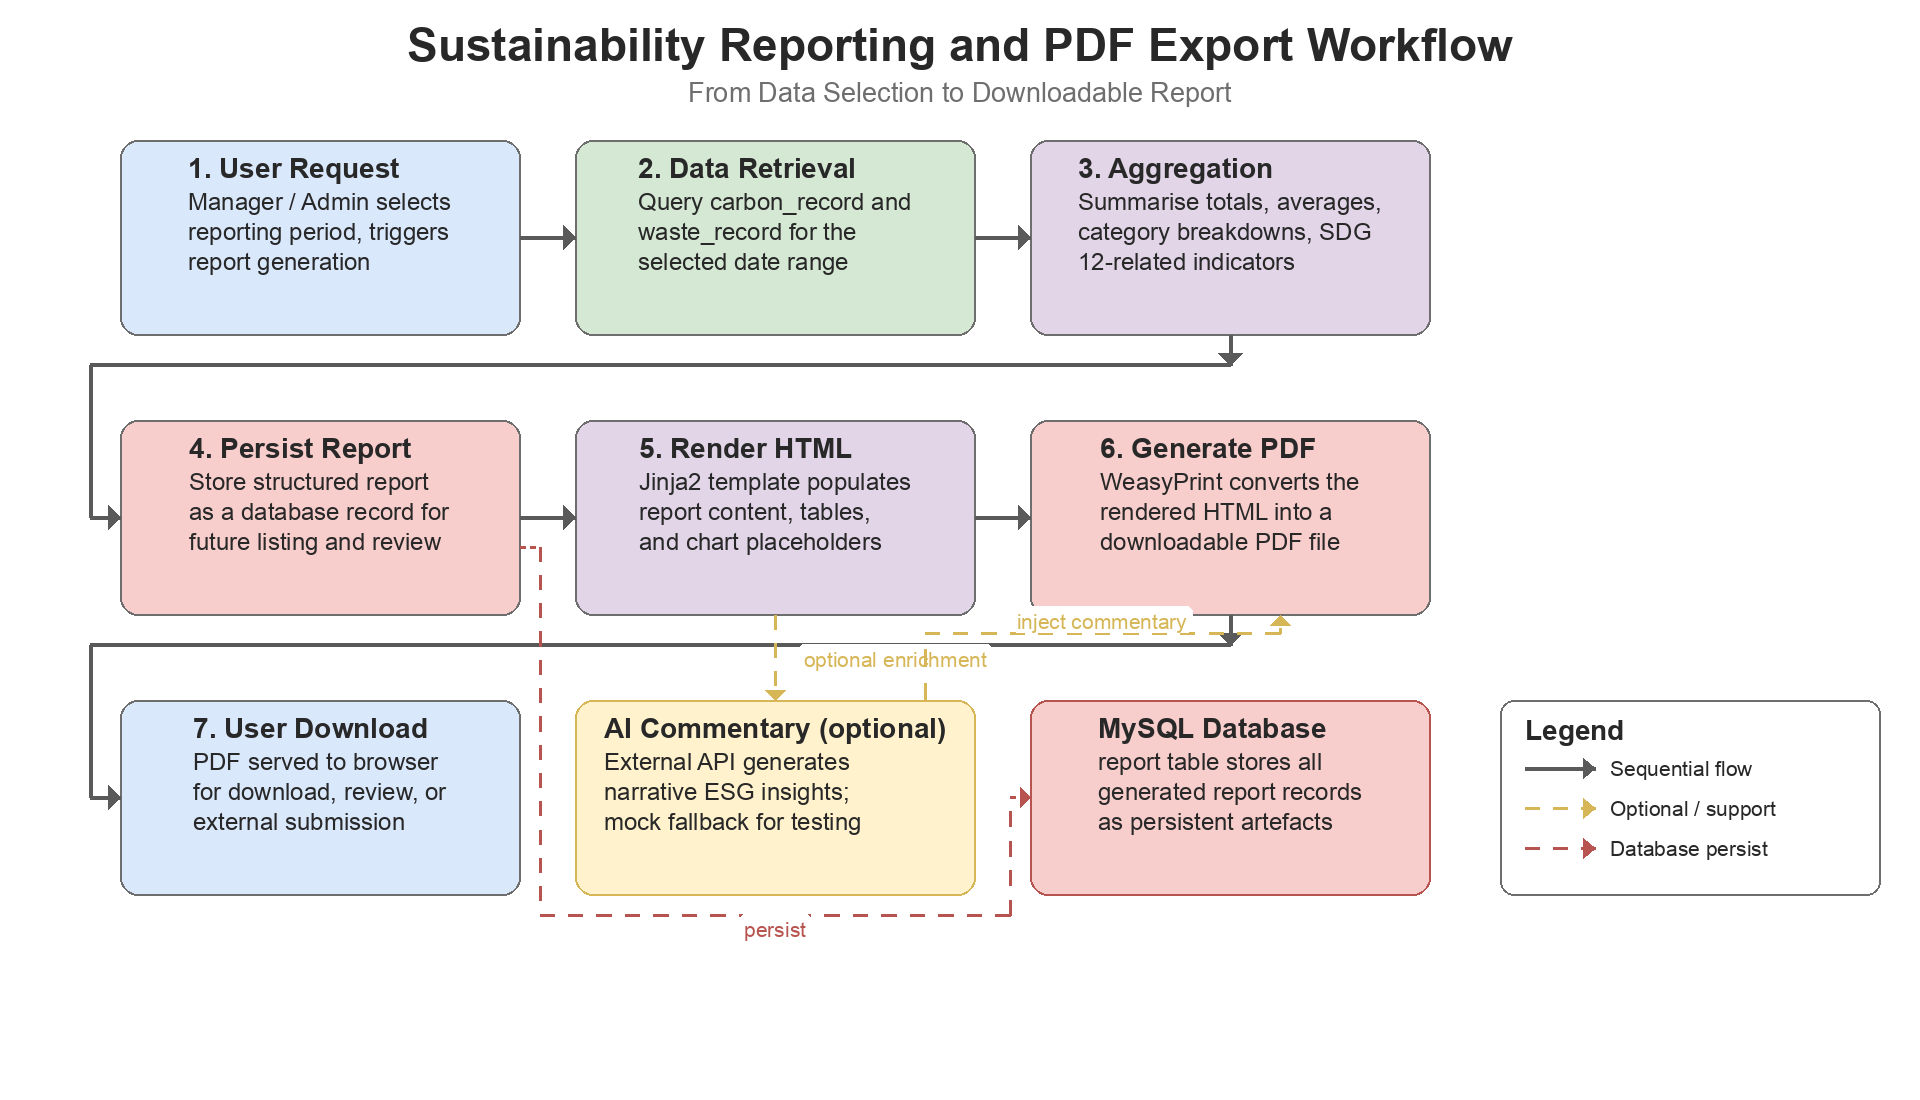
\includegraphics[width=\textwidth]{figures/report_workflow.png}
\caption{Sustainability Reporting and PDF Export Workflow}
\end{figure}

\subsection{Alerts and Notification Mechanism}
The alert subsystem provides threshold-based monitoring for sustainability performance. Users with appropriate permissions can define thresholds for selected metrics at company, region, or store level. When new operational data are processed, relevant alert logic can be triggered and recorded for later review.

\new{Concretely, the \texttt{alert\_threshold} table stores per-threshold configuration: \texttt{metric\_type} (one of three ENUM values \texttt{waste\_recycling\_rate}, \texttt{carbon\_mom\_growth}, \texttt{waste\_weight\_daily}), \texttt{scope} (\texttt{company}, \texttt{region}, or \texttt{store}) with an optional \texttt{scope\_id}, the numeric \texttt{threshold\_value}, a \texttt{comparison} operator (\texttt{lt} or \texttt{gt}), a comma-separated \texttt{notify\_email} list, and an \texttt{is\_active} flag. HQ managers and administrators can create and edit thresholds; region managers and store staff have read-only access. Default thresholds shipped with the platform fire when monthly recycling rate falls below~30\% or when month-on-month carbon growth exceeds~20\%.}

\new{Trigger evaluation is event-driven rather than scheduled. Every successful insert into the carbon or waste record tables ends with a call to a shared alert-checker helper. That helper loads every active threshold for the company, filters by scope, and evaluates the relevant metric: the recycling-rate check sums recycled weight over total weight for the current month; the carbon month-on-month check compares the latest two monthly totals from a per-store summary view; the daily-waste check sums today's waste weight on the store.}

\new{When a threshold is breached, the helper writes an alert log row with the metric snapshot and threshold reference, deduplicating per store, metric, and month so a single recurring breach does not flood the inbox. The frontend surfaces unread alerts through a badge on both the sidebar and the topbar, refreshed every sixty seconds by a JavaScript poll against the unread-count endpoint.}

\new{Email notification is wired through Flask-Mail. A mail helper exposes \texttt{send\_alert\_email()}, which formats a subject of the form ``\texttt{[ESG Alert] <metric label> threshold breached --- <store name>}'' and a plain-text body listing store, metric, current value, threshold, and timestamp. When the application's \texttt{MAIL\_SERVER} configuration key is set---during demonstration we point it at the Mailtrap sandbox (\texttt{sandbox.smtp.mailtrap.io}) so that real outbound delivery is verifiable without spamming inboxes---the message is sent through SMTP. When \texttt{MAIL\_SERVER} is not configured, or when Flask-Mail is not installed in the environment, the helper writes a \texttt{[Mail MOCK]} entry to the server log containing the same fields, so demonstrations still observe what would have been sent. This dual behaviour is what makes the alert subsystem suitable for both real deployment and offline review.}

\subsection{ESG Management Module}
The ESG Management section groups supplier assessment and ESG policy management under one interface, extending the platform from internal store-activity monitoring into governance-oriented sustainability management.

\subsubsection{Supplier ESG Assessment}
The supplier module manages supplier records and evaluates them through a rule-based ESG scorecard with four dimensions---carbon, waste, ethics, and reporting---each containing four sub-indicators scored as 0 (does not meet), 50 (partially meets), or 100 (clearly meets). Weighted aggregation produces both dimension-level scores and an overall grade. The discrete three-level scale keeps each score traceable to a specific sub-indicator, which is both more transparent than a single manual total and more realistic than a data-hungry predictive model for the project context.

\begin{table}[h]
\centering
\scriptsize
\begin{tabularx}{\linewidth}{@{}p{0.15\linewidth}p{0.40\linewidth}p{0.15\linewidth}X@{}}
\toprule
\textbf{Dimension} & \textbf{Example Sub-indicators} & \textbf{Score Options} & \textbf{Purpose} \\
\midrule
Carbon & Disclosure, reduction target, carbon monitoring, supporting evidence & 0 / 50 / 100 & Evaluates whether the supplier tracks and improves carbon-related performance \\
Waste & Waste reduction, recycling practice, disposal control, waste reporting & 0 / 50 / 100 & Captures resource-efficiency and waste-handling responsibility \\
Ethics & Labour practice, compliance awareness, traceability, ethical policy support & 0 / 50 / 100 & Reflects social and governance expectations in supplier behaviour \\
Reporting & ESG disclosure, consistency, completeness, review readiness & 0 / 50 / 100 & Measures the supplier's reporting transparency and management maturity \\
\bottomrule
\end{tabularx}
\caption{Structure of the Supplier ESG Scorecard}
\end{table}

From a workflow perspective, the supplier module supports adding, editing, listing, and deleting supplier records, while automatically recalculating ESG scores whenever data are submitted. Overall scoring uses fixed dimension weights of carbon~0.30, waste~0.30, ethics~0.20, and reporting~0.20, with a final letter grade derived from the weighted total. This removes dependence on manually entered total scores and ensures the overall grade remains aligned with the selected sub-indicator values.

\subsubsection{ESG Policy Management}
Alongside supplier scoring, the ESG Management area also hosts a policy management page that records policy category, version, status lifecycle (draft / active / archived), effective date, and content. This lets the platform represent both ESG evaluation and ESG policy maintenance within one governance space, supporting a clearer connection between governance rules and day-to-day sustainability practice.

\subsection{Training and Compliance Evaluation}
The training module stores sustainability-related training records (course type, completion data, scores, and summary statistics) so that staff capability development is captured as part of ESG management. The compliance score module then aggregates five ESG-relevant dimensions---carbon management, waste and recycling, staff training, reporting frequency, and alert resolution---into a single weighted score, combining operational and managerial signals rather than relying on a single metric.

\begin{table}[h]
\centering
\scriptsize
\begin{tabularx}{\linewidth}{@{}p{0.22\linewidth}p{0.26\linewidth}X@{}}
\toprule
\textbf{Dimension} & \textbf{What It Measures} & \textbf{Main Data Source} \\
\midrule
Carbon Management & Consistency and quality of carbon-related operational records & Carbon tracking records and comparisons \\
Waste and Recycling & Waste handling quality, recycling performance, and recovery-related behaviour & Waste management records and recovery metrics \\
Staff Training & Participation, completion, and coverage of sustainability-related training activity & Training records and summary statistics \\
Reporting Frequency & Whether sustainability reporting is being produced regularly and in usable form & Stored report records and reporting history \\
Alert Resolution & Whether monitored issues are noticed, logged, and followed through at management level & Alert thresholds, alert logs, and review status \\
\bottomrule
\end{tabularx}
\caption{Dimensions Used in ESG Compliance Evaluation}
\end{table}

\new{Each dimension is implemented as a self-contained scoring function in the compliance blueprint, and the per-dimension maxima are deliberately unequal so that the score rewards the modules that carry the most operational signal. The five maxima sum to~100: Carbon Management~30 (half from store coverage of carbon records, half from an intensity penalty that linearly reduces the second half once average monthly carbon exceeds 2{,}000\,kg CO2e per store), Waste \& Recycling~25 (15 points scaling linearly with recycling rate up to a 60\% saturation point plus 10 points for store coverage of waste records), Staff Training~20 (unique trained staff divided by total store staff, multiplied by 20), Reporting Frequency~15 (year-to-date report count divided by the quarterly target of~4, capped at 15), and Alert Resolution~10 (resolved alerts divided by total alerts). The final letter grade is assigned in four bands (A~$\geq$~85, B~$\geq$~70, C~$\geq$~55, D otherwise), and every per-store input passes through \texttt{get\_accessible\_store\_ids()} so each user role sees a score scoped to their own organisational view.}

By calculating a weighted total score and final grade, the platform converts distributed activity across multiple modules into a compact summary that can be read quickly and compared over time, acting as a synthesis layer between operational data quality and governance-oriented performance.

\subsection{Advanced Management and Support Functions}
The platform includes additional modules for data quality assurance, user administration, accountability, and input convenience, each described below.

\subsubsection{Anomaly Detection}
The anomaly detection module applies two complementary strategies to flag unusual carbon and waste records. The statistical approach uses Z-score analysis: for a configurable look-back window (default 90~days), records are grouped by category, and any record whose Z-score exceeds the threshold (default 2.0) is flagged as medium ($|z|\geq2$) or high ($|z|\geq3$) severity. The rule-based approach flags structural impossibilities directly---zero or negative carbon activity values, and waste records where recycled weight exceeds total weight. Table~\ref{tab:anomaly} summarises both methods.

\begin{table}[h]
\centering
\scriptsize
\begin{tabularx}{\linewidth}{@{}p{0.16\linewidth}p{0.12\linewidth}p{0.30\linewidth}X@{}}
\toprule
\textbf{Method} & \textbf{Applies To} & \textbf{Trigger Condition} & \textbf{Severity} \\
\midrule
Z-score (statistical) & Carbon & Per-category total\_carbon deviates $\geq$ threshold $\sigma$ from mean & Medium ($|z|\geq2$); High ($|z|\geq3$) \\
Z-score (statistical) & Waste & Per-category weight\_kg deviates $\geq$ threshold $\sigma$ from mean & Medium ($|z|\geq2$); High ($|z|\geq3$) \\
Rule-based & Carbon & Activity value $\leq$ 0 & High \\
Rule-based & Waste & Recycled kg $>$ total weight kg & High \\
\bottomrule
\end{tabularx}
\caption{Anomaly Detection Methods and Trigger Conditions}
\label{tab:anomaly}
\end{table}

\new{Statistical detection identifies that a record is unusual, but it does not say \emph{why}. To close that gap, the anomaly module includes an optional LLM-backed insight layer.~\footnote{Implemented in \texttt{ai\_insight.py}.} After Z-score and rule-based detection produce the carbon and waste anomaly lists, the top three of each (six items total) are serialised into a strict JSON prompt and sent to DeepSeek in a single round-trip (\texttt{deepseek-chat}, \texttt{max\_tokens=700}, \texttt{temperature=0.4}, 30-second timeout). The prompt instructs the model to return one object per anomaly with a \texttt{risk\_category} drawn from a closed vocabulary (\emph{Data Quality}, \emph{Operational Issue}, or \emph{Fraud Signal}) plus a short markdown insight describing the likely root cause and recommended audit actions. Batching the request and constraining the output schema together keep the per-detection cost manageable and the response parseable.}

\new{The insight layer is wrapped in a defensive fallback. If the API key is missing, the call times out, the response is non-2xx, or the JSON cannot be parsed, the helper silently substitutes a deterministic rule-based insight built from the same anomaly fields. This is what makes the anomaly page usable during offline demonstrations: a reviewer always sees a categorised explanation, with the source distinguished only by an internal \texttt{used\_llm} flag returned in the API response. Persisted insights are stored on the \texttt{anomaly\_review} row (\texttt{ai\_insight}, \texttt{risk\_category}) together with the four-state human triage machine (\emph{Open}, \emph{Reviewed}, \emph{False Positive}, \emph{Resolved}). Re-detection runs only refresh insights for anomalies that are still in the current top-N \emph{and} still \emph{Open}: once a human verdict is recorded the row is preserved, so AI commentary cannot overwrite an auditor's decision.}

\subsubsection{User Management and Audit Logging}
The user management module enables administrators and headquarters managers to create, update, delete, and reset passwords for user accounts within their organisational scope. The system validates username uniqueness, password strength, and role assignment against the four defined system roles, stores passwords using secure hashing, and prevents self-deletion or cross-company modification. Region and store dropdowns are populated dynamically from the organisational hierarchy so role and scope assignments stay consistent. Every management action is recorded in the audit log with the responsible user, target, and IP address.

The audit logging module records significant user actions---logins, record creation, updates, deletions, exports, and administrative operations---into an immutable log table capturing acting user, action type, target entity, IP address, and timestamp. The management page supports filtering by action type, target type, and date range, and a statistics endpoint aggregates action counts over the past seven days. Visibility respects role-based isolation: administrators see all entries, while HQ managers see only their company's. Sensitive fields such as passwords are excluded.

\subsubsection{OCR-Assisted Input}
OCR-assisted bill scanning extracts category, activity value, date, and supplier name from uploaded images or PDFs to prefill the data-entry forms, with a fallback path that keeps the rest of the platform functional when OCR libraries are unavailable.

\new{The OCR pipeline has three layers. The first layer dispatches by extension: image uploads (\texttt{.png}, \texttt{.jpg}, \texttt{.jpeg}, \texttt{.bmp}, \texttt{.tiff}, \texttt{.webp}) are opened with Pillow and passed to \texttt{pytesseract.image\_to\_string()}, while PDF uploads are parsed page-by-page with \texttt{pdfplumber} and concatenated into a single text blob. The second layer is a regex-driven field extractor that runs over the lower-cased text: keyword matching (kWh / electricity, cubic m / m3 / natural gas, km / mileage) decides the carbon category, and then category-specific patterns pull out the numeric activity value. A small set of date patterns covers the three common UK / EU / US formats (``31~March~2026'', ``2026-03-31'', ``03/31/2026''), and an additional regex pulls the invoice number; the supplier name is taken heuristically from the first non-empty line. The third layer is the safety net: if both \texttt{pytesseract} and \texttt{pdfplumber} fail to import (the default on a fresh VM without the system Tesseract binary) or the extracted text is empty, the endpoint returns a structured mock payload so the data-entry form still receives sensible defaults during demonstration. The returned object carries a \texttt{source} field of \texttt{ocr} or \texttt{mock}, which the frontend can display to make it clear to the user whether the values were actually parsed from their upload.}

\subsection{Database, Migration, and Deployment Support}
Schema evolution is handled by versioned migration scripts in \texttt{database/migrations/} (incremental, repeatable, and covering later additions such as ESG scorecard fields), and selected modules---supplier records, policy content, AI commentary, OCR input, and email notification---carry mock fallback paths so demonstrations remain functional when external services or optional dependencies are unavailable.

\new{For demonstration and evaluation we ship a small but realistic dataset. A bundled schema script seeds one company, three regions, and six demo stores distributed across China (Beijing, Guangzhou, Shanghai, Nanjing, Hangzhou) with real geographic coordinates so the map module works out of the box. A separate demo-data seeding script inserts representative waste records for February and March 2026 across all six stores (covering paper cups, plastic packaging, food residue, and coffee grounds with mixed disposal methods) and a training-record set spanning January to April 2026 with the eight course types actually rendered by the training page (carbon awareness, waste management, energy efficiency, green procurement, sustainability reporting, etc.). The data are intentionally not uniform---some stores have higher carbon than others and recycling rates vary---so the dashboard role-specific cards, the anomaly detector, and the compliance score all have something non-trivial to display during the demo.}

The production stack combines Nginx~\cite{nginx} as the reverse proxy in front of a Gunicorn~\cite{gunicorn} worker pool, with HTTPS provisioned through Let's Encrypt and SSH protected by \texttt{fail2ban}.

\new{The deployment target is a UCD-provided Ubuntu~22.04 virtual machine reached at \texttt{csi6220-1-vm2.ucd.ie}. The VM exposes only ports 22, 80, and 443 to the outside, so the application itself binds to \texttt{127.0.0.1} and Nginx acts as the public-facing reverse proxy. The Flask app runs as a Gunicorn worker pool managed by a systemd service unit, which keeps the platform alive across SSH disconnects and reboots; the Nginx site configuration is templated with the VM hostname and project path during the install step. HTTPS is provisioned via Let's Encrypt using \texttt{certbot --nginx}, which also rewrites the Nginx config to redirect HTTP traffic. \texttt{fail2ban} guards the SSH port, and the team uses a tolerant \texttt{maxretry=10}, \texttt{findtime=10m} jail to avoid locking out group members during testing sessions. Configuration values that differ between environments (database credentials, mail server, DeepSeek API key) are loaded from a \texttt{.env} file kept out of source control. This pattern keeps the deployment description short for the report yet realistic enough that the same instructions reproduce on any equivalent Ubuntu VM.}

\subsection{Geographic Map and Region Coverage Visualisation}
\new{The map module is the spatial complement to the dashboard. Where the dashboard reads a store's performance as numbers and trend lines, the map renders the same data as colour-coded markers on a tile-based world map, so that a manager can quickly see at a glance which physical locations are at risk and where coverage is incomplete. The module is implemented as a dedicated blueprint registered as \texttt{map} (page route \texttt{/map}, data routes under \texttt{/api/map}). The store table carries two new columns---\texttt{latitude} and \texttt{longitude}---which were back-filled with real district-level coordinates for the six demo stores; new stores added through the admin UI inherit empty coordinates and are simply excluded from the map until populated, so that incomplete data never produces a misleading dot on the map.}

\new{The data endpoint \texttt{GET /api/map/stores} returns the accessible stores together with summary metrics computed in the same query path used elsewhere in the platform: \texttt{carbon\_ytd\_kg} from \texttt{carbon\_record}, a \texttt{recovery\_rate} that promotes \texttt{disposal\_method} of \emph{recycling}, \emph{composting}, or \emph{reuse} over the legacy \texttt{recycled\_kg} field (matching the ESG-standard definition of waste diverted from landfill), and the open-alert count from \texttt{alert\_log}. A second endpoint \texttt{GET /api/map/store-trend} returns a single store's monthly carbon and recycling trend so the marker popup can show a small sparkline without re-fetching the full dataset. Both endpoints pass store IDs through \texttt{get\_accessible\_store\_ids()}, and \texttt{store-trend} additionally rejects \texttt{store\_id} values outside the caller's accessible set with HTTP 403. Region-level data are aggregated server-side by averaging member-store coordinates so the alternative regions view never exposes the raw store list to a user who is not allowed to see it.}

\new{On the frontend, the page loads Leaflet together with two community plug-ins: \texttt{markercluster} for the dense-marker view and \texttt{heat} for the heatmap overlay. Three modes share the same data: Stores plots each shop as a marker inside the cluster group; Regions plots one large marker per region at its centroid; Heatmap renders carbon intensity as a green--amber--orange--red gradient. Markers are coloured by a coarse three-band grade computed on the server (red when at least three open alerts or recovery rate below 30\%; amber when recovery rate below 50\% or carbon year-to-date above 20{,}000\,kg; green otherwise), and the KPI cards above the map plus the Top-N stores panel react to the same filter set as the markers, so toggling a region or a grade filter keeps every part of the page in agreement.}

\section{Use of Generative AI}
Generative AI tools were used during this project as supporting assistants rather than as replacements for design or implementation decisions. In practice, AI was helpful in four main areas: (1)~coding productivity---suggesting implementations, refactoring ideas, and bug-fix directions; (2)~debugging---interpreting error messages and identifying likely causes; (3)~documentation---improving wording, reorganising content, and expanding technical descriptions; and (4)~design communication---turning rough ideas into clearer specifications that could be compared with the actual codebase.

However, we found that AI output could not be trusted directly. In a Flask project with many blueprints, role-based permissions, and business rules, AI-generated code sometimes ignored the actual database schema, used wrong variable names, or described features that had not been implemented. Similarly, AI-written documentation could blur the line between implemented functions and future extensions, or make a feature sound more mature than it really was. These risks were especially problematic for system documentation, which must describe the real system accurately. We therefore checked all AI-assisted output manually: code suggestions were compared against existing routes, templates, and schema; documentation was verified against actual pages and permission logic; and LaTeX changes were confirmed through local compilation.

Overall, AI improved our development speed and documentation efficiency but did not reduce the need for human judgement. The most reliable approach was to use AI as a reviewer and writing assistant on tasks where we already understood the target module well enough to evaluate the result critically. Prompts that were too open-ended or lacked project context produced more hallucinations. For that reason, our team treated AI as a productivity tool rather than a replacement for technical responsibility, and final acceptance always depended on manual verification.

\new{In the course of building the platform we used AI tools for four concrete tasks where the human cost of doing them manually would have been disproportionate to their value. First, when the LaTeX build kept failing with cryptic fragile-command errors and a recurring soul-package reconstruction failure, the AI reviewer pointed at the interaction between the soul-based revision-highlight macro and certain LaTeX commands within seconds, after which we isolated each offending paragraph and re-ran \texttt{pdflatex} to confirm the cause. Second, the JSON-output prompt for the anomaly insight module went through several iterations of AI-suggested wording before we settled on a strict schema with a closed \texttt{risk\_category} vocabulary, and we verified each iteration by inspecting the live DeepSeek response against the documented contract. Third, the regex set in the OCR endpoint was drafted with AI assistance for the date and invoice-number patterns, and then tested against real bill-style fixtures before being merged. Fourth, AI helped us cross-check the deployment runbook (Nginx + Gunicorn + systemd + certbot + fail2ban) against known good configurations, but the final \texttt{esg.service} unit and \texttt{nginx-esg.conf} were both reviewed line by line on the VM before the production switch. In every case the value of AI came from compressing the search-and-debug loop, not from producing accepted output without inspection.}

\section{Groupwork}
Our project followed a work-package structure, so each member had a main area to focus on, while still helping with integration and later revisions across the system. This worked reasonably well for our team because it gave everyone clear responsibilities without making the work completely separate. As the project developed, several modules became more connected than we expected at the beginning, especially around ESG management, reporting, compliance, and integration. Because of that, the final contribution pattern was not only based on the original work-package plan, but also on the adjustments we made during implementation.

In terms of collaboration workflow, the team used Git for version control and coordinated through regular online meetings. Code reviews were conducted informally within functional pairs (e.g.\ backend and frontend developers reviewing each other's integration points). Documentation tasks were split between two members at a time, with one person drafting content and the other reviewing against the actual codebase. This approach helped reduce inconsistencies and ensured that written descriptions matched the implemented system rather than an idealised version.

\begin{table}[h]
\centering
\scriptsize
\begin{tabularx}{\linewidth}{@{}p{0.06\linewidth}p{0.16\linewidth}p{0.16\linewidth}X@{}}
\toprule
\textbf{WP} & \textbf{Lead} & \textbf{Focus Area} & \textbf{Key Deliverables} \\
\midrule
WP1 & Yao Tianren   & Requirements \& Design  & User analysis, architecture, database design, low-fidelity prototypes \\
WP2 & Liu Haopu     & Backend Development     & API routes, validation, business logic, schema, migrations \\
WP3 & Li Sihang     & Frontend Foundation     & Framework setup, auth UI, reusable components, role-sensitive navigation \\
WP4 & You Haoyang   & Business Frontend       & Carbon/waste/report pages, charts, dashboard, PDF export integration \\
WP5 & Lu Yuan       & Integration \& Testing  & End-to-end flow, compatibility, deployment, performance optimisation \\
WP6 & Liu Haopu     & Delivery \& Documentation & System/user docs, test accounts, VM deployment, presentation \\
\bottomrule
\end{tabularx}
\caption{Work-Package Structure and Responsibilities}
\end{table}

\subsection{Yao Tianren}
Yao Tianren was mainly responsible for WP1, which covered requirements analysis and overall system design. His main contribution was to help define the scope of the project and turn broad sustainability goals into a system structure that could realistically be implemented within one semester. This included analysing the likely needs of business users, identifying key scenarios for carbon tracking, waste management, and sustainability reporting, and helping shape the project into a multi-role ESG management platform rather than just a few separate record pages.

His work covered system architecture, functional decomposition, database structure planning, and low-fidelity design preparation. These early design choices shaped later modules such as ESG policy management, supplier assessment, and the compliance-scoring layout.

\new{He also led the design review for the geographic map module, advising on the three-mode structure (Stores / Regions / Heatmap) and on the server-side three-band grading rule, and helped settle the compliance-score weighting (30 / 25 / 20 / 15 / 10) so that the dimensions reflected the relative operational importance of each module rather than splitting the 100 points evenly. He also reviewed the documentation structure to keep formatting and highlight conventions consistent across all sections.}

\subsection{Liu Haopu}
Liu Haopu was mainly responsible for WP2 and WP6, covering backend development as well as project delivery and final documentation. His main contribution was building the backend foundation of the platform, including database instance preparation, schema construction, API design, validation logic, and business-rule handling across the main functional modules. This included account management, carbon and waste workflows, sustainability reporting, alert processing, ESG management, and other core backend services.

Key technical contributions included the weighted supplier scorecard algorithm, the multi-dimensional compliance scoring engine, the emission-factor-based carbon calculation pipeline, the database migration framework for incremental schema evolution, and final delivery materials (system / user documentation, test accounts, VM deployment, presentation).

\new{He also implemented the bulk CSV / Excel import and export endpoints for the carbon and waste modules using \texttt{pandas}, the four-state anomaly review state machine with the LLM insight layer, the event-driven alert checker that fires after each carbon and waste insert, the database migration that distinguishes AI-generated commentary from rule-based templates on each report, the OCR three-layer extract / regex / mock pipeline, and the map blueprint with its two endpoints. He also produced this system documentation, together with a structured rule set in \texttt{STYLE\_NOTES.md} that captures the soul-package and fragile-command pitfalls discovered during compilation.}

\subsection{Li Sihang}
Li Sihang was mainly responsible for WP3, which focused on the frontend foundation of the system. His main task was to establish the structural base of the interface layer so that later business modules could be developed in a more consistent way. This included frontend framework setup, page organisation, routing-related coordination in the Flask/Jinja environment, reusable UI component preparation, request integration patterns, and general interface consistency.

Specific deliverables included the \texttt{apiFetch} helper for authenticated JSON requests, the shared sidebar and navigation template with role-conditional visibility, the login and registration flow, and the reusable modal and alert components used across all business modules.

\new{He further extended the shared frontend foundation to support the additional modules: the unread-alert badge wired into both the sidebar and the topbar with a 60-second polling interval, the role-conditional visibility rules for the map and anomaly pages, and the consistent toast / modal patterns reused by the bulk CSV import dialogs in the carbon and waste pages. These additions kept the additional business modules visually and behaviourally consistent with the existing pages without forcing a UI redesign.}

\subsection{You Haoyang}
You Haoyang was mainly responsible for WP4, which focused on the implementation of core business-facing frontend modules. His contribution was mainly to turn business requirements into user-facing workflows across the main sustainability functions of the platform. This included carbon-tracking pages, waste-management interfaces, reporting-related interaction, and the visual presentation of data through dashboard components and page-level integration.

Notable technical work included the ECharts-based dashboard visualisations (carbon trend, waste composition, category breakdown charts), the report preview and PDF download flow, the carbon and waste comparison modals, and the supplier scorecard form with dynamic score calculation feedback.

\new{He also rebuilt the dashboard around role-specific cards (the HQ Risk Watch panel, the regional and store cards) and integrated the geographic map page on the frontend, including the Leaflet map initialisation, the three-mode toggle (Stores / Regions / Heatmap), the marker popups with their per-store sparkline served by \texttt{/api/map/store-trend}, and the synchronised KPI / Top-N panels. He also added the bulk CSV / Excel upload UI for the carbon and waste pages, including the row-level error display that surfaces validation messages from the backend.}

\subsection{Lu Yuan}
Lu Yuan was mainly responsible for WP5, which focused on system integration, testing, and deployment-oriented refinement. His main task was to connect the database, backend logic, frontend pages, and business workflows into a usable end-to-end platform. This included identifying module interaction problems, supporting compatibility and integration checks, and improving the overall stability of the system as features were brought together.

Specific contributions included cross-browser compatibility testing, end-to-end workflow validation for all four user roles, network adaptation for remote access from Ireland, performance profiling of database queries, and coordination of the final deployment onto the course VM.

\new{He also owned the production deployment onto the UCD-provided Ubuntu virtual machine: writing the Nginx site configuration and the corresponding systemd unit, provisioning HTTPS through Let's Encrypt with \texttt{certbot --nginx}, tuning the \texttt{fail2ban} jail to a tolerant \texttt{maxretry=10}, \texttt{findtime=10m} so that group testing did not lock anyone out, and producing the demo-data seeding script that loads representative waste and training records used in every demonstration. He also coordinated end-to-end smoke tests across the four user roles after every redeploy.}

\section{Conclusion}
The Business Sustainability Management Platform has developed into a comprehensive system that supports operational record management, role-based access control, dashboard analytics, report generation, alert monitoring, ESG governance workflows, training support, compliance evaluation, anomaly detection, user administration, and audit tracking. One of its main strengths is the combination of everyday business workflows with broader governance and assurance functions: carbon tracking and waste management provide the operational data foundation, while reporting, compliance scoring, supplier assessment, and policy management extend these records into meaningful management processes.

Overall, the current implementation provides a credible and testable ESG platform that reflects both technical development work and business-oriented sustainability management concerns. Although there is room for future extension---such as deeper external data integration or more advanced analytical models\new{, an automated backend test suite based on \texttt{pytest}, a Playwright headless-browser script for the four role-based happy paths, and a GitHub Actions workflow that runs both on every push}---the present version demonstrates a coherent, functional, and well-scoped system suitable for user testing, presentation, and further improvement.

\begin{thebibliography}{9}

\bibitem{gri2021}
Global Reporting Initiative,
\textit{GRI Standards},
GRI, Amsterdam, 2021.
Available: \url{https://www.globalreporting.org/standards/}

\bibitem{eccles2014}
R.~G. Eccles, I.~Ioannou, and G.~Serafeim,
``The Impact of Corporate Sustainability on Organizational Processes and Performance,''
\textit{Management Science}, vol.~60, no.~11, pp.~2835--2857, 2014.

\bibitem{flask2023}
Pallets Projects,
\textit{Flask: Web Development, One Drop at a Time},
2023.
Available: \url{https://flask.palletsprojects.com/}

\bibitem{ghgprotocol}
World Resources Institute and World Business Council for Sustainable Development,
\textit{The Greenhouse Gas Protocol: A Corporate Accounting and Reporting Standard},
Revised Edition, 2004.
Available: \url{https://ghgprotocol.org/}

\bibitem{mysql2024}
Oracle Corporation,
\textit{MySQL 8.0 Reference Manual},
2024.
Available: \url{https://dev.mysql.com/doc/refman/8.0/en/}

\bibitem{iso14064}
International Organization for Standardization,
\textit{ISO 14064-1:2018 -- Greenhouse gases -- Part 1: Specification with guidance at the organization level for quantification and reporting of greenhouse gas emissions and removals},
ISO, Geneva, 2018.

\bibitem{un_sdg12}
United Nations,
``Goal 12: Ensure sustainable consumption and production patterns,''
\textit{Sustainable Development Goals},
2015.
Available: \url{https://sdgs.un.org/goals/goal12}

\bibitem{owasp2021}
OWASP Foundation,
\textit{OWASP Top Ten -- 2021},
2021.
Available: \url{https://owasp.org/www-project-top-ten/}

\bibitem{deepseek2024}
DeepSeek,
\textit{DeepSeek API Documentation -- Chat Completions},
2024.
Available: \url{https://api-docs.deepseek.com/}

\bibitem{leaflet2024}
V.~Agafonkin,
\textit{Leaflet -- An Open-Source JavaScript Library for Mobile-Friendly Interactive Maps}, version 1.9.4,
2024.
Available: \url{https://leafletjs.com/}

\bibitem{markercluster}
D.~Leaver,
\textit{Leaflet.markercluster -- Marker Clustering Plugin for Leaflet}, version 1.5.3,
2023.
Available: \url{https://github.com/Leaflet/Leaflet.markercluster}

\bibitem{weasyprint}
Kozea,
\textit{WeasyPrint -- The Awesome Document Factory},
2024.
Available: \url{https://weasyprint.org/}

\bibitem{pandas2024}
W.~McKinney and the pandas development team,
\textit{pandas: Powerful Python Data Analysis Toolkit},
2024.
Available: \url{https://pandas.pydata.org/}

\bibitem{tesseract}
R.~Smith,
``An Overview of the Tesseract OCR Engine,''
\textit{Proceedings of the 9th International Conference on Document Analysis and Recognition (ICDAR)}, vol.~2, pp.~629--633, 2007.

\bibitem{bootstrap}
M.~Otto, J.~Thornton, and contributors,
\textit{Bootstrap -- The Most Popular HTML, CSS, and JS Framework}, version 5,
2023.
Available: \url{https://getbootstrap.com/}

\bibitem{mee2023}
Ministry of Ecology and Environment of the People's Republic of China,
\textit{Notice on the Management of Greenhouse Gas Emission Reporting for Enterprises in the Power Generation Sector (2023--2025)},
2023.
Available: \url{https://www.mee.gov.cn/}

\bibitem{seai2023}
Sustainable Energy Authority of Ireland,
\textit{Conversion Factors for Energy and Carbon},
2023.
Available: \url{https://www.seai.ie/data-and-insights/seai-statistics/conversion-factors/}

\bibitem{ipcc2023}
Intergovernmental Panel on Climate Change,
\textit{2006 IPCC Guidelines for National Greenhouse Gas Inventories (2019 Refinement)},
IPCC, Geneva, 2019.
Available: \url{https://www.ipcc-nggip.iges.or.jp/public/2019rf/}

\bibitem{defra2023}
UK Department for Environment, Food and Rural Affairs,
\textit{Greenhouse Gas Reporting: Conversion Factors 2023},
2023.
Available: \url{https://www.gov.uk/government/publications/greenhouse-gas-reporting-conversion-factors-2023}

\bibitem{echarts}
Apache Software Foundation,
\textit{Apache ECharts},
version 5, 2024.
Available: \url{https://echarts.apache.org/}

\bibitem{nginx}
F5 / Nginx Inc.,
\textit{nginx Documentation},
2024.
Available: \url{https://nginx.org/en/docs/}

\bibitem{gunicorn}
B.~Chesneau and contributors,
\textit{Gunicorn -- Python WSGI HTTP Server for UNIX},
2024.
Available: \url{https://gunicorn.org/}

\end{thebibliography}

\end{document}
